\section{Durchführung}
\label{sec:Durchführung}
\subsection{Vorbereitungsaufgaben}
\label{sec:vorbereitung}
Die in der Vorbereitungsaufgabe gefragten Literaturwerte bezüglich der Ordnungszahl $Z$, der Energie der K-Kante $E_K$, des Braggwinkels
$\theta_K$ und der Abschirmkonstante $\sigma$ sind im Folgenden tabellarisch dargestellt.
\begin{table}[H]
    \centering
        \caption{Die gefragten Literaturwerte zu verschiedenen Elementen.\cite{AP05}}
        \label{tab:diss1}
        \sisetup{table-format=1.2}
        \begin{tabular}{S S[table-format=2.0] S[table-format=2.2] S[table-format=2.1] S}
          \toprule
          {Element} & {$Z$} & {$E_K [\si{\kilo\electronvolt}]$} & {$\theta [\si{\degree}]$} & {$\sigma$}\\
          \midrule
            {Zn} & 30 & 9.65  & 18.6 & 3.56 \\
            {Ge} & 32 & 11.10 & 18.2 & 3.68 \\
            {Br} & 35 & 14.47 & 15.0 & 3.85 \\
            {Rb} & 37 & 15.20 & 13.3 & 3.95 \\
            {Sr} & 38 & 16.10 & 12.6 & 4.01 \\
            {Zk} & 40 & 17.99 & 11.3 & 4.11 \\
          \bottomrule
        \end{tabular}
      \end{table}
\subsection{Der Versuchsaufbau}
\label{sec:Versuchsaufbau}
Der Veruchsaufbau ist in folgender Grafik zu erkennen.
\begin{figure}[H]
  \centering
  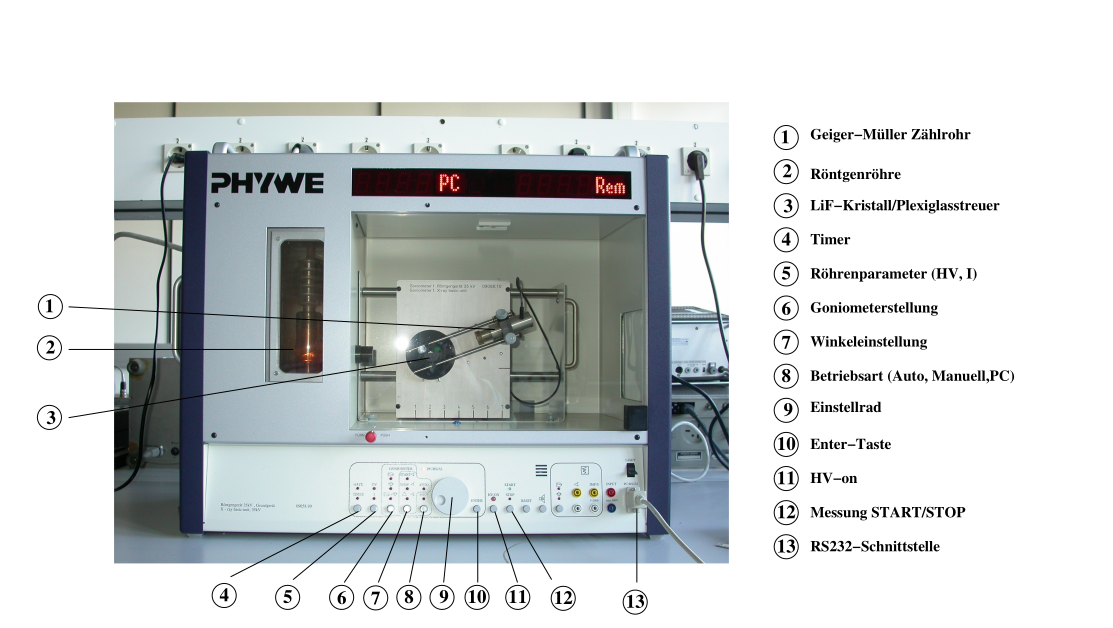
\includegraphics[scale=0.5]{"content/aufbau.png"}
  \caption{Der Versuchsaufbau.}
  \label{fig:aufbaudurchführung}
\end{figure}
\noindent
Der Versuchsaufbau besteht aus einer Kupfer-Röntgenröhre, welche auf einen LiF-Kristall
ausgerichtet ist. Der Kristall lässt sich auf verschiedene Winkel einstellen,
wodurch die Intensität der Röntgenstrahlung sich für verschiedene Glanzwinkel
messen lässt. Zur Intensitätsmessung wird ein Geiger-Müller Zählrohr verwendet.
Die Messung sowie die Winkeleinstellung lassen sich über die Bedienelemente des
Gerätes steuern. 
